% 01 — Script §1, opening.
\sectiontag{1}\source{}
% Revised title page; suppress navigation locally while retaining the footline.
\begingroup
\setbeamertemplate{headline}{}
\begin{frame}[t]
\vspace*{76pt}
{\fontsize{52}{60}\selectfont\bfseries\color{SemBlue} AdvNet\par}
\vspace{18pt}
{\fontsize{30}{38}\selectfont Revealing Performance Issues in Network Protocols\\
by Generating Adversarial Environments\par}
\vspace{48pt}
{\fontsize{24}{30}\selectfont Presenters: Eric Gao and Xiaoyang Chen\par}
\end{frame}
\endgroup

% Revised slides 2--3 follow the slide blueprint and updated script order.
\source{}
\begin{frame}[t]{Background: Congestion Control}
\compactfont
\begin{center}
\begin{tikzpicture}[x=1pt,y=1pt]
\path[use as bounding box] (0,-12) rectangle (880,119);
\node[draw=SemBlue,minimum width=145pt,minimum height=40pt] (s) at (80,66) {Sender};
\node[draw=SemBlue,minimum width=220pt,minimum height=40pt] (q) at (340,66) {Bottleneck queue};
\node[draw=SemBlue,minimum width=145pt,minimum height=40pt] (r) at (800,66) {Receiver};
\draw[flow] (s) -- (q);
\draw[flow] (q) -- node[above=5pt,font=\fontsize{20}{25}\selectfont] {Throughput: achieved rate}
  node[below=5pt,font=\fontsize{20}{25}\selectfont] {Bandwidth: link capacity} (r);
\draw[ack] (r.south) -- (800,0) -- (80,0) -- (s.south);
\node[fill=white,font=\fontsize{20}{25}\selectfont] at (440,0)
  {ACK (acknowledgement) return path};
\end{tikzpicture}
\end{center}
\vspace{-4pt}
{\color{SemBlue}\textbf{Unknown available bandwidth}}\par
\begin{itemize}\setlength{\itemsep}{5pt}
\item Send too slowly $\to$ underutilize bandwidth
\item Send too fast $\to$ queue buildup, higher round-trip time (RTT), packet loss
\end{itemize}
\pause
\vspace{8pt}
{\color{SemBlue}\textbf{Feedback-driven adaptation}}\par
\begin{itemize}\setlength{\itemsep}{5pt}
\item Signals: ACKs, delay, packet loss
\item Controls: congestion window (in-flight limit) and pacing (send timing)
\item Loss recovery: duplicate ACKs and retransmission timeouts (RTO)
\end{itemize}
\end{frame}

\source{}
\begin{frame}[t]{Motivation: Congestion Control Is Hard to Test}
\bodyfont
\vspace{8pt}
{\color{SemBlue}\textbf{Strict goals in dynamic networks}}\par
\begin{points}
\item High throughput, low delay, and low loss under changing links
\item Fast convergence to stable, fair rates when flows compete
\end{points}
{\fontsize{18.5}{22}\selectfont\color{SemGray}
Adapted from PCC Vivace: Online-Learning Congestion Control \S1\par}
\pause
\vspace{24pt}
{\color{SemBlue}\textbf{Consequences for testing}}\par
\begin{points}
\item A large parameter space makes thorough testing difficult.
\item Protocol updates and new designs may pass standard tests\newline
      yet hide severe regressions.
\item Goal: automatically find environments that expose performance problems.
\end{points}
\end{frame}

% Revised slides 4--5: existing tests and prior adversarial testing.
\source{}
\begin{frame}[t]{Motivation: Existing Testing Approaches Fall Short}
\bodyfont
{\color{SemBlue}\textbf{Hand-designed tests}}\par
\begin{itemize}\setlength{\itemsep}{7pt}
\item Manually chosen bandwidth and latency ranges: easy to interpret\newline
      and useful for checking suspected issues
\item Coverage depends on the designer; protocol state makes the\newline
      sequence space grow exponentially with sequence length.
\end{itemize}
\pause
\vspace{16pt}
{\color{SemBlue}\textbf{Real-world traces and testbeds}}\par
\begin{itemize}\setlength{\itemsep}{7pt}
\item Coverage is bounded by collection sites and times.
\item No active search for worst cases; live anomalies are hard to reproduce.
\end{itemize}
\vspace{12pt}
{\labelfont\renewcommand{\arraystretch}{1.2}
\begin{tabularx}{\linewidth}{@{}p{140pt} L@{}}
\toprule
Mahimahi & Record-and-replay link emulator\\
Pantheon & Congestion-control benchmark across real and emulated paths\\
Puffer & Live adaptive video streaming testbed\\
\bottomrule
\end{tabularx}}
\end{frame}

\source{}
\begin{frame}[t]{Adversarial Testing: Simulation vs. Emulation}
\bodyfont
\vspace{12pt}
{\compactfont\renewcommand{\arraystretch}{1.3}
\begin{tabularx}{\linewidth}{@{}p{225pt} L@{}}
\toprule
Simulation (ns-3) & Simplified models: fast and deterministic, but behavior can differ from deployed code.\\
\midrule
Emulation (Mahimahi) & Real OS kernel stack: exposes implementation bugs, but execution is slow and noisy.\\
\bottomrule
\end{tabularx}}\par
\pause
\vspace{18pt}
{\color{SemBlue}\textbf{Prior work: CC-Fuzz}\quad\normalfont (HotNets '22)}\par
\begin{points}
\item Uses a genetic algorithm (GA) in ns-3 simulation.
\item Represents links as low-level Packet Delivery Opportunities (PDOs).
\item Struggles to find strong adversarial examples within a limited emulation budget
\end{points}
\vspace{8pt}
{\fontsize{18}{22}\selectfont\color{SemGray}Will explain later\par}
\end{frame}

% Revised Part 2: architecture, scoring, and design challenges.
% Three-stage architecture walkthrough using the original Figure 1.
\newcommand{\architecturefocus}[1]{%
\begin{tikzpicture}
\node[anchor=south west,inner sep=0pt] (architecture) at (0,0)
{\includegraphics[page=2,trim=251bp 131bp 46bp 486bp,clip,width=620pt]{../docs/AdvNet - Revealing Performance Issues in Network Protocols by Generating Adversarial Environments.pdf}};
\begin{scope}[x={(architecture.south east)},y={(architecture.north west)}]
#1
\end{scope}
\end{tikzpicture}}

\source{Fig. 1, AdvNet.}
\begin{frame}[t]{AdvNet: Inputs and Reference}
\vspace{24pt}
\begin{columns}[c,onlytextwidth]
\column{250pt}
\compactfont
{\color{SemBlue}\textbf{Inputs}}\par
\begin{itemize}\setlength{\itemsep}{7pt}
\item Parameter bounds
\item Target protocol
\item Reference baseline
\end{itemize}
\vspace{22pt}
{\color{SemBlue}\textbf{Reference options}}\par
\vspace{12pt}
{\labelfont
$\left\{\begin{aligned}
&\text{Another protocol}\\
&\text{An older version}\\
&\text{A single-path configuration}\\
&\text{A capacity benchmark}
\end{aligned}\right.$\par}
\column{620pt}
\architecturefocus{
\draw[red,line width=3pt] (.09,.625) ellipse [x radius=.085,y radius=.10];
\draw[red,line width=3pt] (.68,.405) ellipse [x radius=.15,y radius=.035];
}
\end{columns}
\end{frame}

\source{Fig. 1, AdvNet.}
\begin{frame}[t]{AdvNet: Execution Loop}
\vspace{24pt}
\begin{columns}[c,onlytextwidth]
\column{250pt}
\compactfont
\begin{enumerate}\setlength{\itemsep}{16pt}
\item Generate a candidate trace.
\item Run target and reference in the same environment.
\item Score their performance gap and feed it back to the generator.
\end{enumerate}
\vspace{20pt}
{\fontsize{18}{23}\selectfont\color{SemGray}
Mahimahi is extended to support time-varying delay and dual paths.\par}
\column{620pt}
\architecturefocus{
\draw[red,line width=3pt] (.39,.68) ellipse [x radius=.135,y radius=.12];
\draw[red,line width=3pt] (.68,.29) ellipse [x radius=.18,y radius=.26];
\draw[red,line width=3pt] (.14,.39) ellipse [x radius=.075,y radius=.085];
}
\end{columns}
\end{frame}

\source{Fig. 1, AdvNet.}
\begin{frame}[t]{AdvNet: Output Stage}
\vspace{24pt}
\begin{columns}[c,onlytextwidth]
\column{250pt}
\compactfont
{\color{SemBlue}\textbf{Post-Learning Selection}}\par
\vspace{12pt}
\begin{enumerate}\setlength{\itemsep}{16pt}
\item Reserve part of the budget to re-test candidates.
\item Select the trace with the most reliably high average score.
\item Independently re-evaluate the selected trace.
\end{enumerate}
\column{620pt}
\architecturefocus{
\draw[red,line width=3pt] (.68,.88) ellipse [x radius=.12,y radius=.105];
\draw[red,line width=3pt] (.89,.74) ellipse [x radius=.105,y radius=.12];
}
\end{columns}
\end{frame}

% Scoring and utility definitions.
\source{}
\begin{frame}[t]{Scoring the Performance Gap}
\bodyfont
$R$: reference performance\qquad $T$: target performance\par
\vspace{18pt}
{\fontsize{36}{44}\selectfont\centering
$\displaystyle\mathrm{score}=\frac{R-T}{\max(R,T)}$\par}
\vspace{16pt}
\begin{center}
\compactfont Higher metric values are better (e.g., throughput).
\end{center}
\pause
\vspace{14pt}
Reference: 10 Mbps\qquad Target: 2 Mbps\par
\vspace{12pt}
{\fontsize{36}{44}\selectfont\centering
$\displaystyle\mathrm{score}=\frac{10-2}{10}=0.8$\par}
\vspace{18pt}
\begin{itemize}\setlength{\itemsep}{10pt}
\item Lower is better (e.g., completion time): use $T-R$ in the numerator.
\item Score lies in $[-1,1]$; positive scores mean the target underperforms.
\end{itemize}
\end{frame}

\source{}
\begin{frame}[t]{Combining Throughput and Delay}
\bodyfont
\vspace{10pt}
{\fontsize{32}{40}\selectfont\centering
$\displaystyle U=t_{\mathrm{coeff}}\frac{\tau}{\tau_{\max}}
+(1-t_{\mathrm{coeff}})\frac{d_{\min}}{d}$\par}
\vspace{22pt}
{\compactfont
$\tau$: throughput\qquad $d$: average packet delay\par
\vspace{8pt}
$\tau_{\max}$: maximum-throughput benchmark\par
$d_{\min}$: minimum-delay benchmark\par}
\pause
\vspace{22pt}
Throughput weight $t_{\mathrm{coeff}}\in[0,1]$:\par
\vspace{12pt}
{\renewcommand{\arraystretch}{1.25}
\begin{tabularx}{\linewidth}{@{}L L L@{}}
\toprule
$1$: throughput only & $0$: delay only & $0.5$: equal weight\\
\bottomrule
\end{tabularx}\par}
\vspace{24pt}
Compute reference and target utilities using the same benchmarks and weight,\newline
then use them as $R$ and $T$ in the performance-gap score.
\end{frame}

\source{}
\begin{frame}[t]{Two Core Design Challenges}
\bodyfont
{\color{SemBlue}\textbf{Sample efficiency}}\par
\begin{points}
\item Real protocol executions take seconds per evaluation.
\item A large trace space and emulation noise limit the search.
\item Repeating every trace leaves less budget for exploring new ones.
\end{points}
\pause
\vspace{22pt}
{\color{SemBlue}\textbf{Practical usefulness}}\par
\begin{points}
\item Zero bandwidth makes every protocol get zero throughput.
\item Sudden bandwidth increases naturally cause brief underutilization.
\item Meaningful reference comparisons must match the developer's task.
\end{points}
\end{frame}
